\documentclass[12pt,onecolumn,a4paper]{article}
\usepackage{epsfig,graphicx,subfigure,amsthm,amsmath}
\usepackage{color,xcolor}     
\usepackage{xepersian}
\settextfont[Scale=1]{sahel.ttf}
\setlatintextfont[Scale=1]{Times New Roman}
\graphicspath{ {./img/} }



\begin{document}


\title{گزیده و نکات بخش اول، مقدمه\\\lr{"Introductory Statistics" by Wonnacott}} 
\author{مهدی صادق‌زاده قمصری}
\date{بهمن ۹۹}
\maketitle

\section{استدلال جز به کل(استقرا) و کل به جز (استنتاج)} 
استقرا یعنی استدلال کردن برای رسیدن از جز به کل، که در آمار می‌توان به نوعی آن را رسیدن از دانش درباره نمونه به دانشی درباره جامعه دانست.
استنتاج وارون این مسیر است؛ و به استدلال برای رسیدن از کل به جز گفته می‌شود که هم‌ارز آماری آن می‌تواند رسیدن از ویژگی‌های جامعه به ویژگی‌های نمونه باشد.(نمونه گیری؟)
نکته اصلی اینجاست که زمانی میتوانیم از جز به کل برسیم که مسئله ای ساده‌تر از استنتاج اولیه داشته باشیم. یعنی چی؟ مثال:
\begin{align*}
\pi = P \pm error     
\end{align*}
در این معادله ما یک استقرا داریم(ویژگی جامعه میتواند با دقتی از ویژگی نمونه استنباط شود) که خود مبتنی بر یک استنتاج پایه‌ای‌تر است(ویژگی نمونه به ویژگی جامعه نزدیک است). 
در بخش ۲ تا ۵ این کتاب، رویکرد رویکردی استنتاجی‌ست؛ برای مثال مطالعه روی احتمال که خودش روی کاربرد هایی مفید است(مانند نظریه بازی ها) اما فایده مهم‌تر آن این است که میتواند پایه ای برای استنتاج های آماری باشد(بخش های ۷ تا ۱۰). 
در بخش ۶ نیز به این سوال پرداخته میشود که "در ازای یک جامعه مشخص، یک نمونه چه ویژگی هایی دارد؟"
زیرا تنها زمانی میتوان به استنتاج و استنباط های های آماری دیگر پرداخت که این سوال پاسخ داده شود؛ و در بخش های بعدی به این میپردازیم که "چگونه و با چه دقتی میتوان از یک نمونه مشخص درباره جامعه(نامعلوم) استنباط هایی داشت؟" 
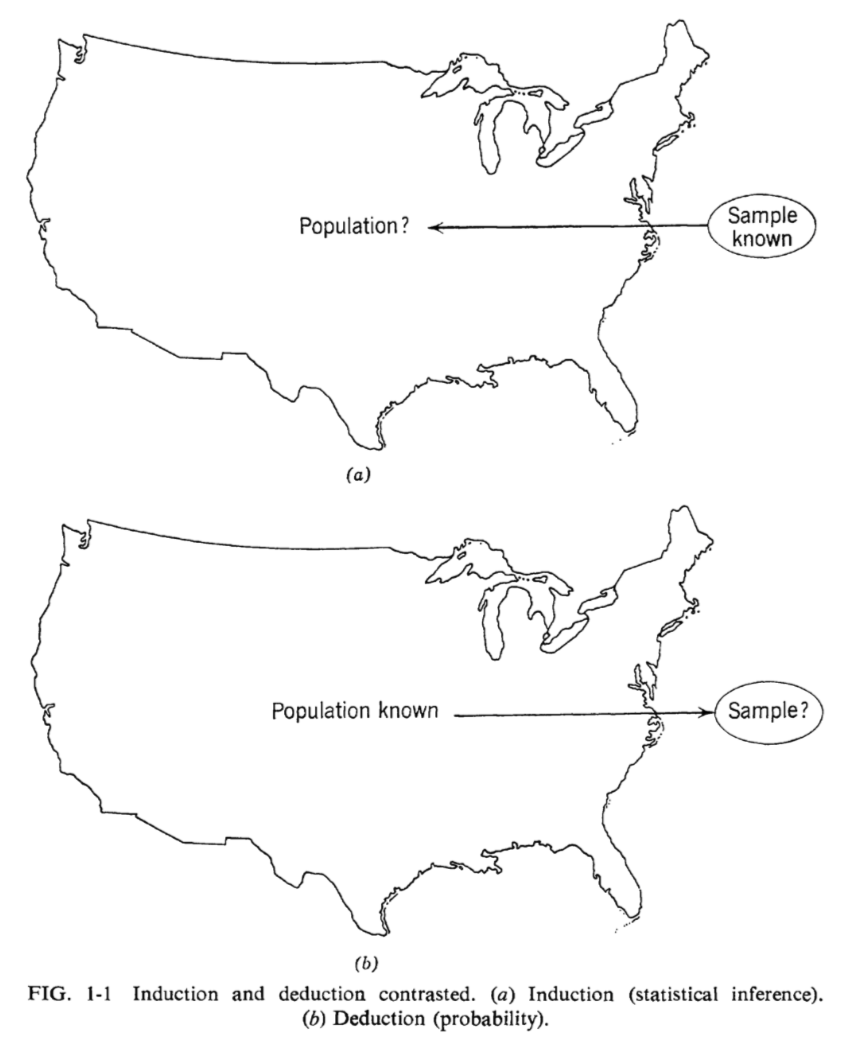
\includegraphics[width=\textwidth]{fig1.png}

\section{چرا نمونه؟}
علت اینکه به بررسی نمونه میپردازیم بجای کل جامعه یکی از ۳ حالت زیر است:
\begin{enumerate}
    \item محدودیت منابع:\\
    به علت بزرگی جامعه، نتوانیم کل آن را مورد بررسی قرار دهیم.
    \item محدودیت داده:\\
    از کل جامعه به مقدار کافی داده موجود نباشد.
    \item آزمایش:\\
    بخواهیم مطلبی را روی جامعه بسنجیم که امکان آزمایش روی همه را نداشته باشیم.
\end{enumerate}

\section{یک نمونه باید چگونه باشد؟}
نمونه نباید سودار یا هدف‌دار جمع‌آوری شود؛ و ساده‌ترین راه برای اطمینان از عدم سوگیری نمونه این است که همه اعضای جامعه احتمال حضور یکسانی در نمونه داشته باشند یا به عبارتی نمونه به طور "تصادفی" انتخاب شود.
در بعضی مواقع ممکن است نتوان نمونه تصادفی داشت یا جمع‌آوری کرد. قضایای نظریه احتمال را مستقیما روی این نمونه ها نمی‌توان به کار برد اما همچنان ممکن است که مبنایی برای  برآورد های علمی بتوان داشت؛ که شاید بتوان به آن نوعی فن استنباط گفت(صرف اینکه بدونیم که همچین چیزایی هم هست).

\end{document}